%%%%%%%%%%%%%%%%%%%%%%%%%%%%%%%%%%%%%%%
% Programming/Coding Assignment
% LaTeX Template
%
% This template has been downloaded from:
% http://www.latextemplates.com
%
% Original author:
% Ted Pavlic (http://www.tedpavlic.com)
%
% Note:
% The \lipsum[#] commands throughout this template generate dummy text
% to fill the template out. These commands should all be removed when 
% writing assignment content.
%
% This template uses a Perl script as an example snippet of code, most other
% languages are also usable. Configure them in the "CODE INCLUSION 
% CONFIGURATION" section.
%
%%%%%%%%%%%%%%%%%%%%%%%%%%%%%%%%%%%%%%%%%

%----------------------------------------------------------------------------------------
%	PACKAGES AND OTHER DOCUMENT CONFIGURATIONS
%----------------------------------------------------------------------------------------

\documentclass[a4paper]{article}

\usepackage{fancyhdr} % Required for custom headers
\usepackage{lastpage} % Required to determine the last page for the footer
\usepackage{extramarks} % Required for headers and footers
\usepackage[usenames,dvipsnames]{color} % Required for custom colors
\usepackage{graphicx} % Required to insert images
\usepackage{listings} % Required for insertion of code
\renewcommand*{\lstlistingname}{代码} % change "Listing <ref> to 代码 <ref>
\usepackage{courier} % Required for the courier font
\usepackage{lipsum} % Used for inserting dummy 'Lorem ipsum' text into the template

\usepackage[UTF8]{ctex} % Required for Chinese character
\usepackage{tocloft} % Required for beautiful toc
\usepackage[colorlinks]{hyperref} % Required for clickable toc
\hypersetup{
    colorlinks=false,
    citecolor=red,
    filecolor=black,
    linkcolor=blue,
    urlcolor=black,
    linkbordercolor	= {1 0 0}
}
\usepackage[title]{appendix} % Required for appendix
\usepackage{float}
\usepackage{amsmath} % used for \text{} in math formula


% used for beautiful table
\usepackage{booktabs} 
\usepackage[T1]{fontenc}
\usepackage{tabu}
\usepackage{longtable}
\usepackage[table]{xcolor}

\usepackage{algpseudocode}
\usepackage{algorithm}

%used for beautiful order list
\usepackage{enumitem}

\def\equationautorefname{式}%
\def\footnoteautorefname{脚注}%
\def\itemautorefname{项}%
\def\figureautorefname{图}%
\def\tableautorefname{表}%
\def\partautorefname{篇}%
\def\appendixautorefname{附录}%
\def\chapterautorefname{章}%
\def\sectionautorefname{节}%
\def\subsectionautorefname{小节}%
\def\subsubsectionautorefname{subsubsection}%
\def\paragraphautorefname{段落}%
\def\subparagraphautorefname{子段落}%
\def\FancyVerbLineautorefname{行}%
\def\theoremautorefname{定理}%
\def\algorithmautorefname{算法}
\let\subsubsectionautorefname\sectionautorefname

% TODO:
\newcommand{\aref}[1]{\hyperref[#1]{附录~\ref{#1}}}

% Margins
\topmargin=-0.45in
\evensidemargin=0in
\oddsidemargin=0in
\textwidth=6.5in
\textheight=9.0in
\headsep=0.25in

\linespread{1.1} % Line spacing

% Set up the header and footer
\pagestyle{fancy}
\lhead{\hmwkAuthorName} % Top left header
\chead{\hmwkClass\ (\hmwkClassInstructor\ \hmwkClassTime): \hmwkTitle} % Top center head
\rhead{\firstxmark} % Top right header
\lfoot{\lastxmark} % Bottom left footer
\cfoot{} % Bottom center footer
\rfoot{Page\ \thepage\ of\ \protect\pageref*{LastPage}} % Bottom right footer
\renewcommand\headrulewidth{0.4pt} % Size of the header rule
\renewcommand\footrulewidth{0.4pt} % Size of the footer rule

\setlength\parindent{0pt} % Removes all indentation from paragraphs

%----------------------------------------------------------------------------------------
%	CODE INCLUSION CONFIGURATION
%----------------------------------------------------------------------------------------

\definecolor{MyDarkGreen}{rgb}{0.0,0.4,0.0} % This is the color used for comments
% \lstloadlanguages{c} % Load Perl syntax for listings, for a list of other languages supported see: ftp://ftp.tex.ac.uk/tex-archive/macros/latex/contrib/listings/listings.pdf
% \lstset{language=sql, % Use Perl in this example
%         frame=single, % Single frame around code
%         basicstyle=\small\ttfamily, % Use small true type font
%         keywordstyle=[1]\color{Blue}, % Perl functions bold and blue
%         keywordstyle=[2]\color{Purple}, % Perl function arguments purple
%         keywordstyle=[3]\color{Blue}\underbar, % Custom functions underlined and blue
%         identifierstyle=, % Nothing special about identifiers                                         
%         commentstyle=\usefont{T1}{pcr}{m}{sl}\color{MyDarkGreen}\small, % Comments small dark green courier font
%         stringstyle=\color{Purple}, % Strings are purple
%         showstringspaces=false, % Don't put marks in string spaces
%         tabsize=4, % 5 spaces per tab
%         %
%         % Put standard Perl functions not included in the default language here
%         % morekeywords={rand},
%         morekeywords={rand, go},
%         %
%         % Put Perl function parameters here
%         morekeywords=[2]{REAL},
%         %
%         % Put user defined functions here
%         morekeywords=[3]{},
%        	%
%         morecomment=[l][\color{Blue}]{...}, % Line continuation (...) like blue comment
%         numbers=left, % Line numbers on left
%         firstnumber=1, % Line numbers start with line 1
%         numberstyle=\tiny\color{Blue}, % Line numbers are blue and small
%         stepnumber=2, % Line numbers go in steps of 5,
%         firstnumber=1
% }

\lstloadlanguages{C++}
\lstdefinestyle{mycpp}{
    language=C++, % Use Perl in this example
    frame=single, % Single frame around code
    basicstyle=\small\ttfamily, % Use small true type font
    keywordstyle=[1]\color{Blue}, % Perl functions bold and blue
    keywordstyle=[2]\color{Purple}, % Perl function arguments purple
    keywordstyle=[3]\color{Blue}\underbar, % Custom functions underlined and blue
    keywordstyle=[4]\color{Aquamarine}, % Custom functions underlined and blue
    identifierstyle=, % Nothing special about identifiers                                         
    commentstyle=\usefont{T1}{pcr}{m}{sl}\color{MyDarkGreen}\small, % Comments small dark green courier font
    stringstyle=\color{Purple}, % Strings are purple
    showstringspaces=false, % Don't put marks in string spaces
    tabsize=4, % 5 spaces per tab
    %
    % Put standard Perl functions not included in the default language here
    % morekeywords={rand},
    morekeywords={go, REFERENCES, DATABASE, SCHEMA, u64},
    %
    % Put Perl function parameters here
    morekeywords=[4]{np},
    %
    % Put user defined functions here
    morekeywords=[1]{self},
    morekeywords=[3]{},
    %
    morecomment=[l][\color{Blue}]{...}, % Line continuation (...) like blue comment
    numbers=left, % Line numbers on left
    firstnumber=1, % Line numbers start with line 1
    numberstyle=\tiny\color{Blue}, % Line numbers are blue and small
    stepnumber=2, % Line numbers go in steps of 5,
    firstnumber=1
}
% Creates a new command to include a perl script, the first parameter is the filename of the script (without .pl), the second parameter is the caption

\newcommand{\shfilescript}[3]{
\begin{itemize}
\item[]\lstinputlisting[caption=#2, label=lst:#1, language=sh]{#3}
\end{itemize}
}
\newcommand{\shscript}[3]{
\begin{itemize}
\item[]\begin{lstlisting}[label=lst:#1, caption=#2] #3 \end{lstlisting}
\end{itemize}
}

%----------------------------------------------------------------------------------------
%	DOCUMENT STRUCTURE COMMANDS
%	Skip this unless you know what you're doing
%----------------------------------------------------------------------------------------

% Header and footer for when a page split occurs within a problem environment
\newcommand{\enterProblemHeader}[1]{
\nobreak\extramarks{#1}{#1 见下页\ldots}\nobreak{} 
\nobreak\extramarks{接上页}{#1 见下页\ldots}\nobreak{}
}

% Header and footer for when a page split occurs between problem environments
\newcommand{\exitProblemHeader}[1]{
\nobreak\extramarks{接上页}{#1 见下页\ldots}\nobreak{}
\nobreak\extramarks{#1}{}\nobreak{}
}
% TODO:code here enable the number before section, but it disable the numbering of problems
%\setcounter{secnumdepth}{0} % Removes default section numbers
\newcounter{homeworkProblemCounter} % Creates a counter to keep track of the number of problems

\newcommand{\homeworkProblemName}{}
\newenvironment{homeworkProblem}[1][Problem \arabic{homeworkProblemCounter}]{ % Makes a new environment called homeworkProblem which takes 1 argument (custom name) but the default is "Problem #"
\stepcounter{homeworkProblemCounter} % Increase counter for number of problems
\renewcommand{\homeworkProblemName}{#1} % Assign \homeworkProblemName the name of the problem
\section{\homeworkProblemName} % Make a section in the document with the custom problem count
\enterProblemHeader{\homeworkProblemName} % Header and footer within the environment
}{
\exitProblemHeader{\homeworkProblemName} % Header and footer after the environment
}

\newcommand{\problemAnswer}[1]{ % Defines the problem answer command with the content as the only argument
\noindent\framebox[\columnwidth][c]{\begin{minipage}{0.98\columnwidth}#1\end{minipage}} % Makes the box around the problem answer and puts the content inside
}

\newcommand{\homeworkSectionName}{}
\newenvironment{homeworkSection}[1]{ % New environment for sections within homework problems, takes 1 argument - the name of the section
\renewcommand{\homeworkSectionName}{#1} % Assign \homeworkSectionName to the name of the section from the environment argument
\subsection{\homeworkSectionName} % Make a subsection with the custom name of the subsection
\enterProblemHeader{\homeworkProblemName\ [\homeworkSectionName]} % Header and footer within the environment
}{
\enterProblemHeader{\homeworkProblemName} % Header and footer after the environment
}


\newcommand{\codev}[1]{\textsf{#1}}
%----------------------------------------------------------------------------------------
%	NAME AND CLASS SECTION
%----------------------------------------------------------------------------------------

% table color
\definecolor{tableHeader}{RGB}{245, 245, 245}
\definecolor{tableLineOne}{RGB}{245, 245, 245}
\definecolor{tableLineTwo}{RGB}{224, 224, 224}
\newcommand{\tableHeaderStyle}{
    \rowfont{\leavevmode\color{white}\bfseries}
    \rowcolor{tableHeader}
}

%----------------------------------------------------------------------------------------

\newcommand{\hmwkTitle}{project-name\ \#2} % Assignment title
\newcommand{\hmwkDueDate}{Tuesday,\ September\ 18,\ 2018} % Due date
\newcommand{\hmwkClass}{16级计科\ 7班} % Course/class
\newcommand{\hmwkClassTime}{周三3-4节} % Class/lecture time
\newcommand{\hmwkClassInstructor}{teacher-name} % Teacher/lecturer
\newcommand{\hmwkAuthorName}{颜彬} % Your name
\newcommand{\hmwkAuthorId}{16337269} % Your id 

%----------------------------------------------------------------------------------------
%	TITLE PAGE
%----------------------------------------------------------------------------------------

\usepackage{titling}

\title{
\vspace{2in}
\textmd{\textbf{\hmwkClass:\ \hmwkTitle}}\\
\normalsize\vspace{0.1in}\small{Due\ on\ \hmwkDueDate}\\
\vspace{0.1in}\large{\textit{\hmwkClassInstructor\ \hmwkClassTime}}
\vspace{3in}
}

\author{\textbf{\LARGE{\hmwkAuthorName}} \\ \\ \textbf{\LARGE{\hmwkAuthorId}}}
\date{} % Insert date here if you want it to appear below your name
%----------------------------------------------------------------------------------------

\begin{document}
% \begin{titlingpage} % This is for ignore page number in first page. package titling

\maketitle

%----------------------------------------------------------------------------------------
%	TABLE OF CONTENTS
%----------------------------------------------------------------------------------------

% \setcounter{tocdepth}{2} % Uncomment this line if you don't want subsections listed in the ToC
% set depth in toc

% \renewcommand{\cftsecleader}{\cftdotfill{\cftdotsep}} % used for dots between <section> and <page>

\renewcommand{\contentsname}{Content} % force the word to be "content
\newpage
\tableofcontents
\addtocontents{toc}{~\hfill\textbf{Page}\par}
\newpage

% below are document body


% To have just one problem per page, simply put a \clearpage after each problem
\section{具体贡献}
在本次期末项目中,我为黑白棋游戏实现了以下的几个功能。
\begin{itemize}
    \item 二进制棋盘压缩及其状态维护
    \item 进一步剪枝的alpha-beta算法
    \item 提出了8种不同的评价指标
    \item 自我博弈的进化算法
\end{itemize}
以上几个功能相辅相成,他们可以共同配合让黑白棋获得更大的棋力。除此之外,以上的许多功能
可以为组员带来便利。例如二进制的棋盘压缩方法大大加快了棋盘维护速度,相当于变相加速了
其它的所有算法。\\

\emph{NOTE: 以上功能使用C++完成,没有基于任何第三方库。}
\subsection{二进制棋盘压缩}
在本次期末项目中,棋盘是8*8的。如果用一个bit表示棋盘上是否有棋子,那么刚好unsigned long long类型(64位)
恰好可以存储棋盘的棋子信息。\\

二进制棋盘压缩方法利用了上述的特点。它用一个u64类型的整数表示黑棋在棋盘中的位置,用另一个
u64整数表示白棋在棋盘中的位置,利用位运算提取棋盘中的所有信息。\\

二进制棋盘压缩方法面临的困难问题是,如何在二进制下高效地取得可下子点,如何高效实现
棋盘的翻转。除此之外,还有有二进制下如何计算黑白棋子个数、计算棋盘空位、判断游戏
是否结束等问题。\\

得益于位运算的优化,基于压缩棋盘的alpha-beta剪枝获得了极大的加速。这一加速也为其他
算法提供了很好的条件。
\subsection{进一步剪枝的alpha-beta算法}
alpha-beta算法可以被进一步优化。注意到游戏在进入中盘后,每一方的可下子点数都很大。
alpha-beta算法的运行速度会在中盘明显地下降。\\

为了解决这个问题,可以对alpha-beta算法进行进一步剪枝。具体思路是,先对所有可行点
做一次很浅的alpha-beta剪枝,然后对所有可行点的估值作排序。排好序后,筛掉一部分估值
很低的顶点,按估值降序继续alpha-beta的搜索过程。\\

这个放在对前期和后期会带来略微的性能下降,可是却能大大加快中盘的搜索速度。
\subsection{8种不同的评价指标}
我为黑白棋的估值总结了8种不同的方法。这些几种估值方法从不同的方面估计棋盘的局势。
他们是
\begin{enumerate}
    \item 估值表估值法
    \item 基于4个角的估值
    \item 靠近角估值
    \item 基于行动力的估值
    \item 基于棋子边缘的估值
    \item 基于棋子个数的估值
    \item 基于半稳定子的估值
    \item 棋盘边界估值
\end{enumerate}
后文会详细介绍这些估值法的具体含义,并给出有效的实现方法。\\

\emph{NOTE: 实际上,最终的估值方法是以上所有估值的加权平均。权重由进化算法
学习得到。} \\

这几种估值方法抽象成了接口,可以为组员提供很大的帮助。例如,这些估值可以作为神经网络
的额外输入,或者作为提供给资源的额外评价指标。
\subsection{自我博弈进化算法}
在提除了alpha-beta剪枝和7种估值法后,应该如何权衡这7种估值法呢?最好的方法是
为7种估值方法提供一个权重,用加权求和的方法得到最终的估值。\\


加权求和有个难点,需要手动确定权重。于是我采用了自我博弈方法和进化方法。方法
大致是
\begin{enumerate}[label=(\alph*)]
    \item 认为给定一个初始权重
    \item 基于最好的权重(第一轮迭代时是初始权重),产生一系列新的权重
    \item 对这些不同权重得到的估值方式进行相互博弈
    \item 选出最好的权重方案,跳转到(b)
\end{enumerate}
这个算法还有很多细节,会在随后解释。最终,各个参数应该会收敛到某一个确定的值。
\section{二进制棋盘压缩}
\subsection{棋盘的表示}
使用两个64位的无符号整数来存储棋盘的信息。每个u64整数有64个bit,每个bit代表8*8棋盘
中的一位。如果该bit是1,代表该位置有棋子。\\

用第一个u64代表黑棋的分布,用第二个代表白棋的分布。用两个整数的\emph{位或}代表已经
下列棋子的位置。
\begin{figure}[!hbt]
    \begin{center}
    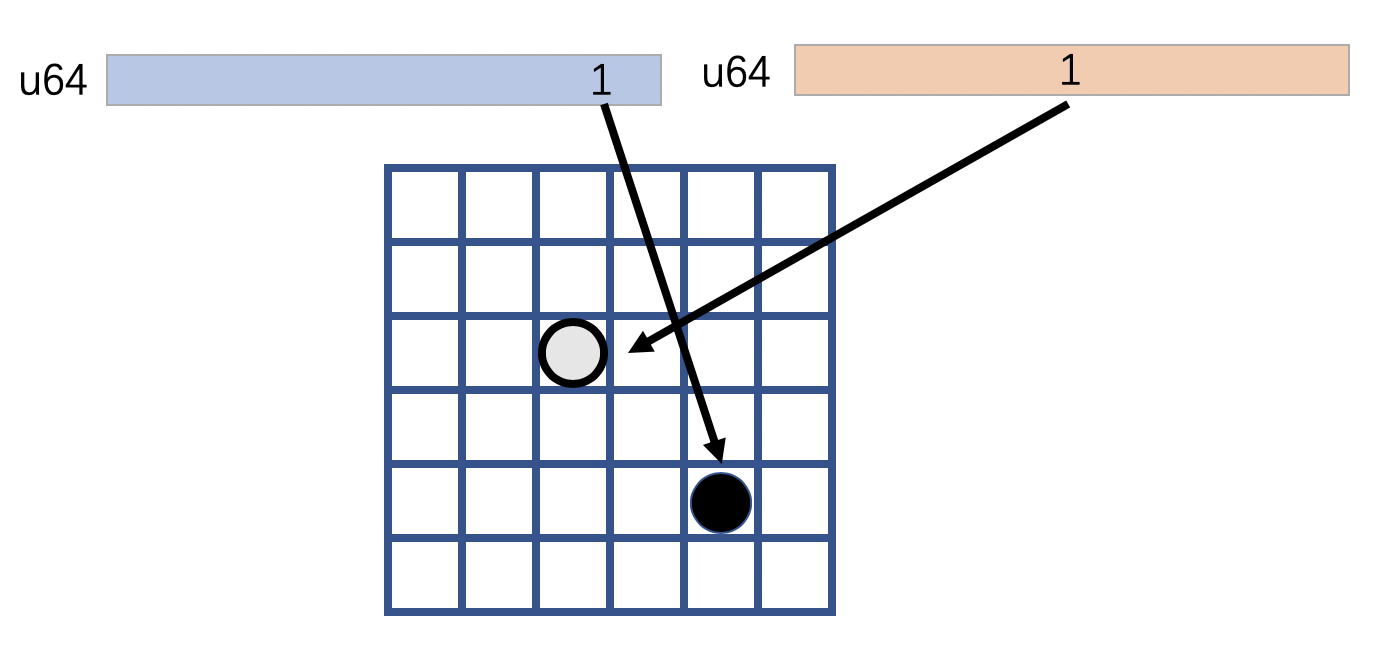
\includegraphics[scale=0.4]{assets/ill.png}
    \caption{二进制表示示意图\label{fig:label}} 
    \end{center} 
\end{figure} 


\subsection{基本的信息提取}
棋盘类必须为其他模块提供必要的接口,他们的实现方法如下。\\

在\autoref{tab:binary-table}中,boards的类型为u64[2]。第一个元素代表黑棋的
棋盘,第二个元素代表白棋的棋盘。参数sq是一个整数,取值范围是[0, 64),代表棋盘的第i位。
参数p是整数,取值范围是\{0, 1\}, 分别代表黑棋和白棋。
\begin{table}[!htb]
\caption{必要接口的二进制实现}\label{tab:binary-table}
\centering
\begin{tabular}{@{} *5l @{}}
    \toprule
\emph{函数} & \emph{参数} & \emph{实现}&& \\
    \midrule
    isEmpty  & sq & ((boards[0] | boards[1]) >> sq) \& 1 \\
    isMyPiece & sq, p & (boards[p] >> sq) \& 1 \\
    isOppPiece & sq, p & (boards[!p] >> sq) \&  1 \\
    \bottomrule
\hline
\end{tabular}
\end{table}

这些方案很好理解。为了确定棋盘的第sq位置是否有棋子,只需要将棋盘右移sq位,然后检查最低位
是否为1。

\subsection{数子个数 - 编译器优化}
可以使用GCC的编译器内置函数\_\_builtin\_popcountll来计算一个整数的二进制中1的个数。\\

这个函数可以为我们计算出棋盘上棋子的个数(1的个数)。而且速度极快。

\subsection{得到可下子点}
得到可下子点的代码如\autoref{lst:movable}所示。\\

定义了一个辅助函数MOVABLE\_HELPER。它是一个宏,接受一个``方向''(例如N)。它的作用
举例来描述。\\

例如在调用MOVABLE\_HELPER(N)时,会首先对自己的棋盘的所有子向上移动一个单位。移动后
与对方的棋子做位与,然后与临时变量作位或。这一步结束后,临时变量存的值代表着,自己的棋子
向上一个单位后碰到的对方棋子位置。\\

对这个行动重复8次(实际上不需要8次,只需要5次,细节在这里省去)。这时临时变量存储的是,
自己的棋子都向上移动1, 2, 3, 4, 5, 6, 7, 8个单位后,碰到的对方的棋子。\\

最后把临时变量向上移动一个单位,并对棋盘的空位做与运算。得到的就是所有可下子的位置。\\

MOVABLE\_HELPER(N)计算的是,``向上''得到的所有的可下子点。对MOVABLE\_HELPER在
8个方向上各做一次,得到的就是整个棋盘的所有下子点。
\begin{figure}[!hbt]
\begin{itemize}
\item[] \begin{lstlisting}[style=mycpp, label=lst:movable, caption=得到可下子点的具体代码]
#define MOVABLE_HELPER(dir) \
    tmp = dir(cur) & opp; \
    for (int i = 0; i < 5; ++i) { \
        tmp |= dir(tmp) & opp; \
    } \
    ret |= dir(tmp) & empty;

inline u64 ChessBox::getMovable(int p) const {
    u64 empty = getEmpty();
    u64 tmp, ret = 0;
    u64 cur = boards[p];
    u64 opp = boards[!p];

    MOVABLE_HELPER(N);
    MOVABLE_HELPER(S);
    MOVABLE_HELPER(W);
    MOVABLE_HELPER(E);
    MOVABLE_HELPER(NW);
    MOVABLE_HELPER(NE);
    MOVABLE_HELPER(SW);
    MOVABLE_HELPER(SE);

    return ret;
}
\end{lstlisting}
\end{itemize}
\end{figure}

\subsection{棋盘翻转}
实现二进制棋盘的下子翻转是一件有一定难度的事情。如代码\autoref{lst:reverte}所示。\\

FLIP\_HELPER接受一个方向,把下的子的那个方向上的所有可翻转的棋子都翻转过来。下面
用一个例子来解释。\\

假设调用了FLIP\_HELPER(N),即考虑下了一个子后,翻转它上方的子。
\begin{itemize}
    \item if语句首先判断这个子的上方是否有对方的子。
    \item 如果有,则不断地将这个子向上移动i单位(i为1, 2, 3, ..., 8),并把这个位置的
对方的子\emph{标记}。
    \item 如果向上移动$i'$个单位后,这个位置没有对方的子,则跳出循环。
    \item 循环结束时,如果位置$i'$上有是自己的子,那么中途所有被标记的位置都要被翻转。
\end{itemize}
上述可以实现上方的子的翻转。对8个方向类似地调用8次,即可翻转所有需要翻转的子。

\begin{figure}[!hbt]
\begin{itemize}
\item[] \begin{lstlisting}[style=mycpp, label=lst:reverte, caption=二进制棋盘的翻转实现]
#define FLIP_HELPER(dir) \
    if (dir(1ull << sq) & opp) { \
        mask = 0; \
        tmp = dir(1ull << sq); \
        for (; tmp & opp;tmp = dir(tmp)) { \
            mask |= tmp; \
        } \
        if (tmp & cur) { \
            cur ^= mask; \
            opp ^= mask; \
        } \
    }

void ChessBox::__flip(int sq, int p) {
    assert(p == BLACK_ID || p == WHITE_ID);
    u64 mask, tmp;
    u64& cur = boards[p];
    u64& opp = boards[!p];

    FLIP_HELPER(N);
    FLIP_HELPER(S);
    FLIP_HELPER(E);
    FLIP_HELPER(W);
    FLIP_HELPER(NE);
    FLIP_HELPER(NW);
    FLIP_HELPER(SE);
    FLIP_HELPER(SW);
}
\end{lstlisting}
\end{itemize}
\end{figure}

\begin{figure}[!hbt]
    \begin{center}
    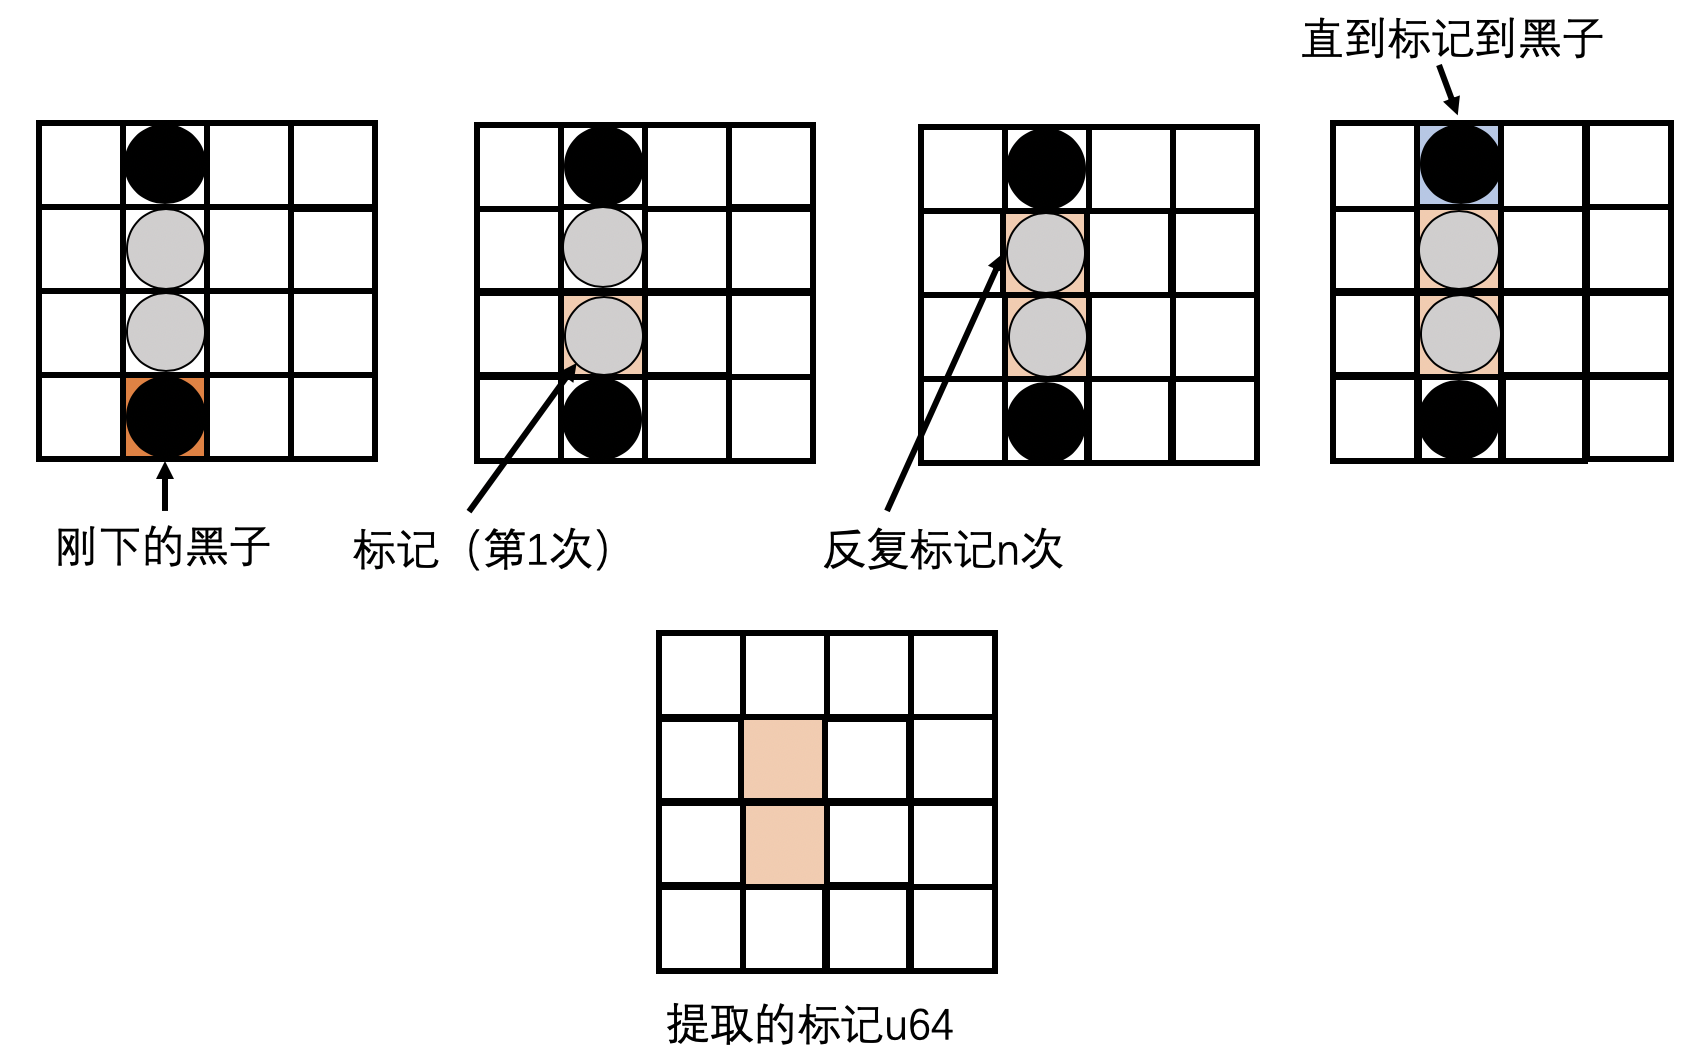
\includegraphics[scale=0.4]{assets/revert.png}
    \caption{棋盘翻转示意图(向上方向)\label{fig:revert}} 
    \end{center} 
\end{figure} 
为了更具体地解释怎么做棋盘反转,可以参考\autoref{fig:revert}。\\

假设黑子下了深橙色标注的下方位置。算法需要单独地考虑8个方向。
假设考虑向上翻转。算法会不断地查看下子位置向上移动一格的那个位置。如果那个位置
是对方的棋子,就进行标记。反复地重复上述过程(如左图三),把上方的一系列对方棋子
进行标记。直到遇到了自己的棋子或标记。\\

如果遇到了自己的棋子,就把标记位提取出来。如果遇到了空位置或边界位置,则把
标志位清空。对双方的棋子按标记位做异或,就完成了一次棋盘的更新。

\subsection{进一步剪枝的alpha-beta算法}
\subsubsection{辅助函数}\label{subsec:ab-trunc-helper}
alpha-beta剪枝的minimax算法可以被进一步地剪枝。
其中用到的辅助函数如\autoref{lst:searchhelper}所示。\\

这个函数的工作是,对棋盘cb,以player为当前玩家,以depth为搜索深度,\emph{返回n个}估值最优的行动方法。
这个n一般很小,这个函数相当于做了一次预筛选。\\

这个函数本质做的也是alpha-beta剪枝。首先它要获取所有可行的下子方式,然后对这些下子方式
做alpha-beta剪枝的minimax算法。然后将他们和他们的最终估值存入候选人列表candidates中。\\

然后,根据当前玩家是黑棋还是白棋,对候选人列表做排序。取有序列表中的前n个元素作为
返回的可行点。\\

\begin{figure}[!hbt]
\begin{itemize}
\item[] \begin{lstlisting}[style=mycpp, label=lst:searchhelper, caption=行动方案预筛选函数]
vector<int> AlphaBetaSolve::search_helper(const ChessBox& cb, 
    int n, int player, int depth) const {
    vector<int> moves = cb.movessq(player);
    vector<Position> candidates;
    for (int move : moves) {
        ChessBox ncb(cb);
        ncb.drop(move/8, move%8, player);
        double ret = alphabeta(ncb, depth, -INF, INF, !player, false);
        candidates.emplace_back(move / 8, move % 8, ret);
    }
    if (player == BLACK_ID) {
        sort(candidates.begin(), candidates.end(), blackPosCmp);
    } else {
        assert(player == WHITE_ID);
        sort(candidates.begin(), candidates.end(), whitePosCmp);
    }
    vector<int> new_moves;
    for (int i = 0; i < n && i < candidates.size(); ++i) {
        new_moves.push_back(candidates[i].x * 8 + candidates[i].y);
    }
    return new_moves;
}
\end{lstlisting}
\end{itemize}
\end{figure}

\subsection{剪枝具体方案}
一般而言,alpha-beta的minimax算法会搜索8层。在这8层搜索的搜索中,搜索前3层时可以
采用\autoref{subsec:ab-trunc-helper}提到的剪枝策略。\\

在这前三层的搜索中,设s表示当前层的可行数。取$$r = \max \{\lfloor s / 2 \rfloor, 3\}$$
r为当前层应该最终应该搜索的分支数。\\

利用上面提到的辅助函数,取n=r,即可得到估值相对较好的
r个分支。只对这r个分支做完整的搜索。\\

一般而言,在调用辅助函数进行预搜索时,预搜索的层数应该比较小。在项目中,预搜索采用的
深度是本来深度的一半。

\section{评价指标}
本实验中,提出了7种不同的评价指标和他们的快速计算方式。
\subsection{估值表估值法}
估值表估值的方法很简单。对于8*8的棋盘,给出一个8*8的估值表。对每个位置,如果这个位置
有棋子,则获得该位置的分数(分数可能是负的)。最后整个棋盘所有位置的分数和就是该玩家的分数。\\

估值表的设置如\autoref{lst:grade}所示。四个角的分数是比较高的。但与4个角相邻的
12个位置的分数却是比较低的。这是因为如果想要占领角的位置,就应该让靠近角的位置让
别人来占领,这样自己就可以通过下子翻转的方式来占领角。\\

边的估值也是比较高的。这是因为当占领了边后,一般而言是比较稳定的。\\

\begin{figure}[!hbt]
\begin{itemize}
\item[] \begin{lstlisting}[style=mycpp, label=lst:grade, caption=估值表的设置]
const int VALUE[8*8] = {
    20, -3, 11,  8,  8, 11, -3, 20,
    -3, -7, -4,  1,  1, -4, -7, -3,
    11, -4,  2,  2,  2,  2, -4, 11,
    8,  1,  2, -3, -3,  2,  1,  8,
    8,  1,  2, -3, -3,  2,  1,  8,
    11, -4,  2,  2,  2,  2, -4, 11,
    -3, -7, -4,  1,  1, -4, -7, -3,
    20, -3, 11,  8,  8, 11, -3, 20,
};
\end{lstlisting}
\end{itemize}
\end{figure}

\subsection{角和临近角估值}
角估值的方法很简单。先统计自己占领的角的数量$n$。再统计对方占领的角的数量$n'$。 
则$c(n - n')$就是当前局面的评分。其中c是一个常数,在这里中取为25。\\

\emph{NOTE: c取25的原因是让取值范围在[-100, 100]里。}\\

临近角的估值方法也很简单。如果一个角没有被占领,那么相邻这个角的3个位置都是坏的位置。
统计自己占领的坏位置的数量$b$和对方的数量$b'$。那么$c(b - b')$就是当前局面的评分。其中c
仍然是一个常数,在这里取为8.3。\\

\emph{NOTE: c取25的原因是让取值范围在[-100, 100]里。}\\

\subsection{棋子数目估值}
棋子数目估值方法十分直接。直接统计棋盘上自己的棋子数和对方的棋子数。算出自己所占
棋子数的百分比。将百分比* 100作为估值。\\

这个估值方法很直接,实际上效果并不好(接下来会看到)。\\

\subsection{行动力估值}
行动力估值的方法是,计算出自己和对方的行动力。算出自己的行动力的百分比。
将行动力的百分比 * 100作为估值。 \\

一般而言,行动力越大越好。这是因为,如果将对手的行动力限制住,对手将
无子可下。最终对手的每一步都会在你的掌控之中。这一方面限制了对手的行动,
另一方面也让自己的搜索结点数大大减小,搜索速度更快。有一举两得的效果。\\

自己的行动力大带来的好处是选择多,则更有可能搜索出能翻盘的结点。

\subsection{边缘棋子数估值}
首先要定义边缘棋子。如果一个棋子有一个一个边暴露在外面,那么这个棋子是
边缘棋子。一般来说,边缘棋子越多,形式越不利。\\

边缘棋子估值的方法是,计算自己的边缘棋子和对方的边缘棋子的占比。返回
自己的边缘棋子百分比 * 100。

\subsection{边界棋子数估值}
边界棋子指的是贴着棋盘的边界的棋子。一般来说,边界棋子越多,局面越好。\\

边界棋子数估值采用的方法是,计算自己和对方的边界棋子的占比。返回
百分比 * 100。

\subsection{半稳定子估值}
半稳定子指的是有一端不可能为对方棋子的子。例如贴着棋盘边缘的棋子,从棋盘的角
斜着延伸到棋盘中部的一系列棋子,等等。\\

半稳定子判断有个好处。第一个是,半稳定子往往比较稳定,半稳定子越多,往往局面优势
越大。除此之外,半稳定子的计算方式十分简单快速。\\

\autoref{lst:halfstable}展示的是玩家p的稳定子的计算方式。其中cur是u64,代表
玩家p的下棋信息。tmp是临时变量,ret是返回值。\\

对于HALF\_STABLE\_HELPER的每次调用,例如HALF\_STABLE\_HELPER(N),它的步骤如下
\begin{enumerate}[label=(\alph*)]
    \item 取得棋盘的所有边界子(与棋盘的边界相邻的子)。记入tmp
    \item 将所有的边界子向上平移一个单位,与自己的棋子位置项与。结果与tmp相或。
    \item 反复(b)3次。
    \item 将结果与ret相或
\end{enumerate}
如此得到的ret即是棋盘上的所有半稳定子。\\

采用半稳定子的个数差的值来估计局面。

\begin{figure}[!hbt]
\begin{itemize}
\item[] \begin{lstlisting}[style=mycpp, label=lst:halfstable, caption=半稳定子的计算方式]
#define HALF_STABLE_HELPER(dir, who) \
    tmp = who & BORDER; \
    for (int i = 0; i < 3; ++i) { \
        tmp |= dir(tmp) & who; \
    } \
    ret |= tmp;

double HalfStableEval::eval(const ChessBox& cb, int p) const {
    // p first
    u64 cur = cb.__getBoard(p);
    u64 tmp, ret = 0;
    HALF_STABLE_HELPER(N, cur);
    HALF_STABLE_HELPER(S, cur);
    HALF_STABLE_HELPER(E, cur);
    HALF_STABLE_HELPER(W, cur);
    HALF_STABLE_HELPER(NE, cur);
    HALF_STABLE_HELPER(NW, cur);
    HALF_STABLE_HELPER(SE, cur);
    HALF_STABLE_HELPER(SW, cur);
    int my_bonus = __builtin_popcountll(ret);
    // ...
}
\end{lstlisting}
\end{itemize}
\end{figure}

\subsection{综合估值}\label{subsec:sum}
综合估值是这里最重要的估值。\\

综合估值会结合上述7种估值方法。综合估值会给每种估值方法一个权重。然后
对这些估值方法做加权求和。\\

加权求和的权重不是认为给定的,是通过进化算法学习得到的。见下文的介绍。

\section{自我博弈的进化算法}
\subsection{大致思路}
一开始,选定一个初始的权重。根据这个权重,随机地产生若干个不同的权重。
利用这些不同的权重产生\emph{综合估值}函数(\autoref{subsec:sum})。\\

利用这些估值函数进行两两对抗。以游戏结束后子的数量差(而不仅仅是胜利和失败)
来评价估值函数的优劣。取出最优的估值函数(获胜后,拉开最大的棋子差的函数),
用这个估值函数的权重来产生数量更多的其他权重。再让他们进行对抗。\\

不断反复上面的这个过程。最终能通过自学习的方法达到最好的权重。

\subsection{细节介绍}
每一轮的进化,共产生4个新的权重,一共组成5个不同的权重。让i和j在[0, 5)这个范围内遍历,对于i != j
的情况(共20种),每种对应一次对弈。其中(i, j)指i为黑方,j为白方进行的对弈。由于训练程序跑在32核
的电脑上,足够开很多的线程,故对弈采用20线程实现。\\

在每次对弈中,共进行6轮比赛。记录每次比赛中i比j多的棋子数,把胜利的棋子数(可能为负)记录在
一个战绩表中。\\

等20次对弈的6轮比赛都完成时,查看战绩表,选中战绩最好的一个权重。不断地利用战绩最好的权重为
初始权重进行新一轮的进化。\\

有一个细节是,战绩表会被多个线程同时修改,所以需要加锁。加锁不会让程序运行速度变慢很多。这是因为
程序的性能瓶颈在对弈。读写是很少的操作。
\subsubsection{结果展示}
在自我博弈的过程中,记录每一轮中获胜子数最多的权重。把获胜字数最多的权重的权重曲线
绘制出来,如\autoref{fig:rev}所示。\\

图左一是将全部估值权重绘制在同一个图片中的场景。图右一是去掉两个最高的曲线后,剩下的
其他估值的权重曲线。\\

值得一提的是,曲线的高低并不能代表这个估值的重要性高低。因为取消只是表示一个估值方法
的权重。而估值方法本身的取值范围是不相等的。例如在棋子个数的估值中,棋子个数估值本身
的取值范围是-100到100。但半稳定子估值中,取值范围是-384到384。如果算法认为这两个
估值的重要性相同,棋子个数估值的权重应该是半稳定子估值的三倍。\\

\begin{figure}[!hbt]
\begin{minipage}{0.48\textwidth}
    \centering
    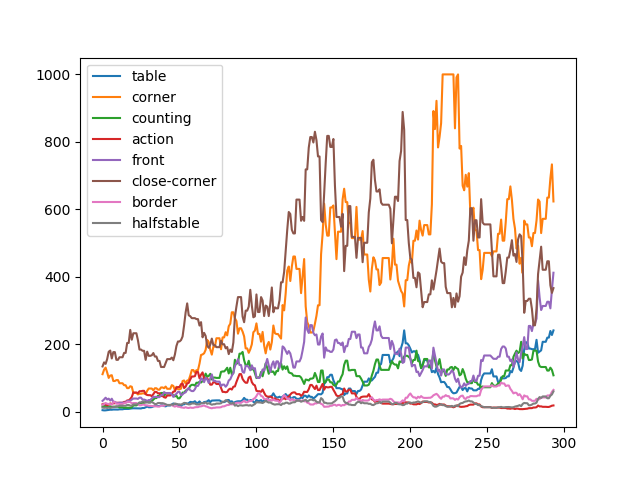
\includegraphics[width=\linewidth]{assets/all.png}
\end{minipage}\hfill
\begin{minipage}{0.48\textwidth}
    \centering
    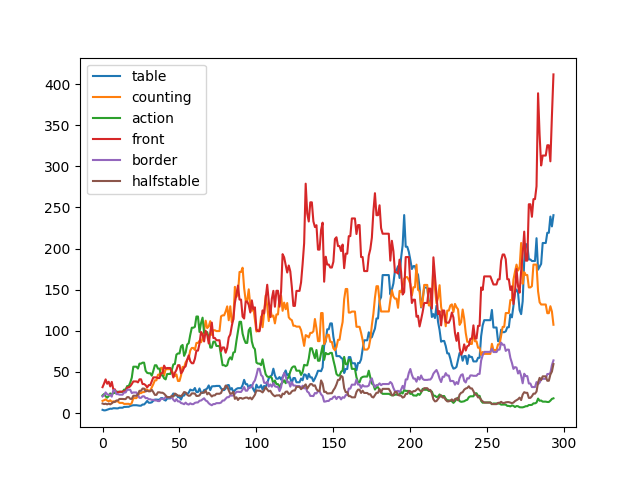
\includegraphics[width=\linewidth]{assets/small.png}
\end{minipage}
\caption{进化算法的权重走势图} \label{fig:rev}
\end{figure}

仔细观察\autoref{fig:rev},会发现一些很有意思的事情。corner估值(橙色)和
close-corner估值(棕色)这两条曲线有一些特殊的关系。首先,corner估值给角落
的四个子以很高的分数,close-corner估值给靠近角落的12个子以很高的分数。这两个
估值的目标是相同的。\\

\emph{如果想要占领角,就要让对方先占领靠近角的12个子。角的重要性越高,
靠近角的12个子的不重要性就越高。}\\

我们可以推断出,corner和close-corner估值是一对\emph{协同估值}。在\autoref{fig:rev}上
,反映成两条曲线是相反的。在曲线1达到峰值时,曲线2达到低估,反之亦然。换言之,
两条曲线的求和是一条比较稳定的直线。\\

这说明我们的进化算法产生了一定的作用,它的确学习到了某些重要的点。它明确了占角
这个行为的重要程度,并且时刻控制着占角的整体的重要性。

\subsubsection{遇到的困难}
在第一次进行进化算法时,我犯了个严重的错误。我的更新方式是,产生随机数$r = rand() \% 20 - 10$,
然后再对原来的权重作$val *= 1 + r * 0.01$。但是我后来发现,这样做之后,val的值是会逐渐变大的。
因为以上的产生随机数的方法中,最大值是10,最小值是-10。不断地反复做1 * 1.1 * 0.9之后,
会发现值实际上是不断变大的。\\

后来我的解决方法是,$r = rand() \% 37 - 17$。这是基于$1 = 1 * 1.2 * 0.83$。这样做
就能保证每个值在多次运算后,结果大致不变。\\

为什么以上的这个细节很重要呢,是因为各个权重值的初始大小是不相等的,例如一个权重值
为10000,可能另一个权重值一开始仅为10。以上的错误会导致偏差,而且偏差会在大的权重
中更明显地反应出来,而在小的权重中不明显地反应。故这就会造成了在迭代一段时间后,
原本较大的估值权重被大大地加大。整个估值体系仅由大估值决定。\\

除了这个问题以外,还需要做的一个细节上的优化是,如果某个权重在进化的过程中超过了
1000,就把它削减成1000。因为估值权重的绝对值是不重要的, 只有权重的比值才是
重要的。如果所有权重同时乘以2,估值效果不变。我试过在进化中,所有权重不断地加大,
直到超过了1e10。这可能导致溢出等不好的结果发生。

\end{document}
